% To translators: don't bother to translate this... english-only version.

\begin{center}
\LARGE{} This is my own bulletin board \normalsize{}
\end{center}

My dear readers! From time to time, I have questions, I don't know who (or where) to ask.
Or I'm just lazy...
Can you please help me?

\myhrule{}

What does tilde means in versions number in .dsc files, which describing Ubuntu packages?
Some kind of wildcard?
And what does \verb|>>| means?
Pipe is just \emph{OR}?
For example:

\begin{lstlisting}
Build-Depends: cython-dbg | python-pyrex, ca-certificates, debhelper (>> 8.1.0~), python (>= 2.6.6-3), python-all-dev (>= 2.6.6-3), python-all-dbg (>= 2.6.6-3), python-configobj (>= 4.7.2+ds-2), python-docutils, python-paramiko, python-pycurl-dbg, python-subunit, python-testtools (>= 0.9.5~)
\end{lstlisting}

\myhrule{}

I have a set of sets.

Some of them intersects with each other, some are not: (a,b,c) (b,c,d) (x,z) (z,y)

I want to group interesting ones, so the output will be: (a,b,c,d) (x,y,z)

What is the proper formal name for such an operation?

\myhrule{}

A delivery service company (like FedEx or UPS) uses 10 (decimal) digit tracking numbers.
Numbers are often transmitten by phone, scribbled on scraps of paper, etc.
You can add, say, 2-3 more (decimal) digits to add some redundancy, so the 10-digit code would be restored
if one digit was transmitten incorrectly.
How to do it?

\myhrule{}

Is there a formal name for such a graphs, that are somewhat similar to codeflow graphs?
They are also planar.
And has some kind of "nested" structure.

\begin{figure}[H]
\centering
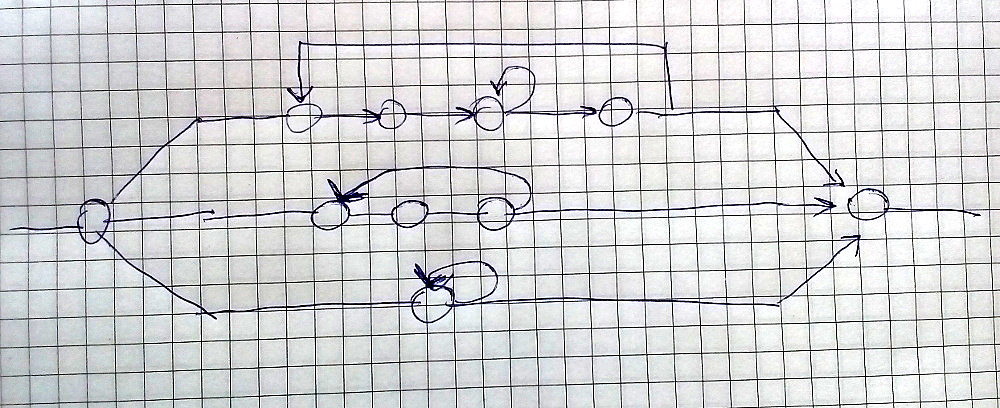
\includegraphics[width=\textwidth]{1st_page}
\caption{A graph}
\end{figure}

\myhrule{}

If you know something, please help me: dennis@yurichev.com

